% -*- latex -*-

\chapter{Customizing Compositing}
\label{chap:Customizing_Compositing}

If you have been reading this document from the beginning, then you already
know enough to use \IceT for many typical rendering applications.  Chapters
\ref{chap:Tutorial} and \ref{chap:Basic_Usage} describe how to build and
link \IceT, establish an \IceT context in your application, and to leverage
\IceT to make your rendering parallel.  This chapter describes the many
features \IceT provides to let you customize the image compositing to your
application.

\section{Compositing Operation}
\label{sec:Customizing_Compositing:Compositing_Operation}
\index{compositing|(}
\index{compositing~operation|(}

\IceT is classified as a \index{sort-last}\keyterm{sort-last} type of
parallel rendering library, as discussed in
Chapter~\ref{sec:Introduction:Parallel_Rendering_Primer}.  Basically, this
means that each process renders images independently, and then these
images, each comprising a different partition of the geometry, are combined
together in a process called \keyterm{compositing}.

To combine two images together, a \keyterm{compositing operation} is
applied to every corresponding pair of pixels.  Three or more images are
combined by applying the compositing operation multiple times to eventually
reduce everything to one image.  (The compositing operations supported by
\IceT are associative, so order does not matter.  \IceT takes advantage of
this fact to efficiently perform the compositing in parallel.)

\IceT supports two compositing operations.  The first type of compositing
operation is a depth comparison and the other is an alpha blend.    The
depth comparison is a bit faster and is easier to use, but only works for
opaque surfaces.  If you are performing
\index{volume~rendering}\keyterm{volume rendering}, the translucent
rendering of 3-dimensional volumes, or any other rendering that involves
transparent data, then you will have to use the alpha blend compositing
operation.

\subsection{Z-Buffer Compositing}
\label{sec:Customizing_Compositing:User_Defined_Communicators}
\index{z-buffer}
\index{z-buffer|seealso{compositing, z-buffer}}
\index{depth~buffer|see{compositing, z-buffer}}
\index{compositing!z-buffer|(}

\keyterm{Z-buffer compositing} takes advantage of the same hidden surface
removal already taking place in the OpenGL pipeline.  \IceT pulls the
\index{z-buffer}z-buffer (also often known as the \keyterm{depth buffer})
from the OpenGL image buffers.  The compositing operation then just
compares the depth values of two pixels and chooses the one that is closer.

Z-buffer compositing is used whenever the depth buffer is chosen as one of
the input buffers.  The input (and output) buffers are chosen with the
\CFunc{icetInputOutputBuffers} function.

\begin{Table}{3}
  \textC{void }\CFunc{icetInputOutputBuffers}\textC{(}&\textC{GLenum}&\CArg{inputs}\textC{,} \\
  &\textC{GLenum}&\CArg{outputs}\quad\textC{);}
\end{Table}

By default, both the the color and the depth buffer are selected as input
buffers and the color buffer is selected as the only output buffer.  This
means that the depth buffer will be used to do z-buffer compositing, but
only the color buffer will be fully composited.  (Not computing the depth
buffer may save some network transfer time.)

If you need the depth buffer composited in addition to the color buffer
(for example, to help with a picking operation), you can do so by simply
setting the depth buffer as one of the output buffers.
\begin{code}
  icetInputOutputBuffers(ICET_COLOR_BUFFER_BIT | ICET_DEPTH_BUFFER_BIT,
                         ICET_COLOR_BUFFER_BIT | ICET_DEPTH_BUFFER_BIT);
\end{code}
Alternatively, if you only need the depth buffer (for example, as a shadow
map), you can do so by setting both the input and output buffers to just
the depth buffer.
\begin{code}
  icetInputOutputBuffers(ICET_DEPTH_BUFFER_BIT, ICET_DEPTH_BUFFER_BIT);
\end{code}

\index{compositing!z-buffer|)}

\subsection{Volume Rendering (and Other Transparent Objects)}
\label{sec:Customizing_Compositing:Volume_Rendering}
\index{blending|see{compositing, blended}}
\index{compositing!blended|(}
\index{volume~rendering|(}

A well known limitation to z-buffer compositing --- and the z-buffer hidden
surface removal algorithm in general --- is that it only works with opaque
objects.  You will get invalid results if you try to apply z-buffer
compositing on transparent objects.

There are two fundamental problems with the z-buffer compositing operation
when dealing with translucent pixels.  The first problem is that you cannot
simply pick the nearest color value.  You must \keyterm{blend} the front
pixel's color with the back pixel's color.  The second problem is that the
color blending is order dependent.  That is, you have to know which pixels
are in front of others.  Although it is technically possible to use
z-buffer values to determine the ordering of a pair of pixels, making sure
that all the pixels get composited in the correct order requires additional
information about and constraints on the geometry.

When z-buffer compositing is not applicable, you must use \keyterm{blended
  compositing}.  Blended compositing is automatically turned on when there
is no z-buffer specified as an input buffer.  That generally means you will
be setting both the input and output buffers to the color buffer.
\begin{code}
  icetInputOutputBuffers(ICET_COLOR_BUFFER_BIT, ICET_COLOR_BUFFER_BIT);
\end{code}

The blending composite operator relies on the \index{alpha}\keyterm{alpha}
(\index{$\alpha$}\keyterm{$\alpha$}) channel of the color buffer (the A in
RGBA colors).  Note that the alpha values must actually be available in the
OpenGL color buffers in order for blended compositing to work.  Many
applications create OpenGL buffers without alpha bit planes in them because
they are often not necessary to render images in serial.  Make sure your
application creates alpha bit planes before attempting to composite
translucent images with \IceT (or any other library).

The blending operation is the standard
\index{over~operator}\index{under~operator}\keyterm{over/under operator}
defined in the seminal 1984 Porter and Duff paper.
\begin{equation}
  C_o \leftarrow C_f + C_b (1 - \alpha_f)
  \label{eq:VolumeRendering:OverOperator}
\end{equation}
where $C$ is an RGBA color vector, $\alpha$ is the alpha component of a
color vector, and the $f$, $b$, and $o$ subscripts denote the front, back,
and output values, respectively.

Each color in Equation~\ref{eq:VolumeRendering:OverOperator} represents a
\index{pre-multiplied~color}\keyterm{pre-multiplied color}, meaning that
the red, green, and blue values are scaled by the alpha parameter.  Thus, a
fully red color at half transparency is represented by the vector $\langle
0.5, 0, 0, 0.5 \rangle$ rather than $\langle 1, 0, 0, 0.5 \rangle$.  In
pre-multiplied colors, none of the red, green, or blue values ever exceed
the alpha value.  Note that colors are often provided in OpenGL as
non-pre-multiplied values, and the blending equation $C_o \leftarrow C_f
\alpha_f + C_b (1 - \alpha_f)$ is used instead of the one in
Equation~\ref{eq:VolumeRendering:OverOperator}.  Although this blending
gives the correct RGB color, it computes an invalid alpha parameter, so
watch out!

\index{ordered compositing|see{compositing, ordered}}
\index{compositing!ordered|(}

Simply turning on blended compositing is not sufficient to render
translucent objects.  You must also tell \IceT to perform \keyterm{ordered
  compositing}.  In ordered compositing, you must have a
\index{visibility~ordering}\keyterm{visibility ordering}.  Given any two
processes, a visibility ordering ensures and determines that all of the
geometry in one process is in front of or behind all the geometry in each
of the other process with respect to the camera.  In some cases, such as
when volume rendering a 3D Cartesian grid of points distributed in blocks
to processes, finding the visibility ordering is straightforward.  In other
cases, such as when rendering unstructured collections of polygons or
polyhedra, it can be difficult to ensure that a visibility ordering exists
and can be found.  Doing so may be the most challenging part of creating a
parallel rendering application.  An example of creating a visibility
ordering from unstructured data can be found in the ParaView application,
and the implementation is detailed in the following paper:

\begin{quote}
  Kenneth Moreland, Lisa Avila, and Lee Ann Fisk. ``Parallel Unstructured
  Volume Rendering in ParaView,'' In \emph{Visualization and Data Analysis
    2007, Proceedings of SPIE-IS\&T Electronic Imaging}, January 2007,
  pp. 64950F-1--12.
\end{quote}

Ordered compositing is turned on by simply passing the
\CEnum{ICET\_ORDERED\_COMPOSITE} flag to \CFunc{icetEnable}.
\begin{code}
  icetEnable(ICET_ORDERED_COMPOSITE);
\end{code}

Once ordered compositing is enabled, it is very important to use
\CFunc{icetCompositeOrder} to specify the visibility order of the geometry
associated with each process.  This must generally be done before each call
to \CFunc{icetDrawFrame}.
\begin{Table}{1}
  \textC{void }\CFunc{icetCompositeOrder}\textC{(} \textC{const GLint *}
  \CArg{process\_ranks} \textC{);}
\end{Table}
The \CFunc{icetCompositeOrder} function takes an array of processes.  It is
assumed that the geometry of the first process in the list is in front of
the rest of the processes; the geometry of the second process in the list
is in front of all the processes except the first, and so on.  The
visibility order often changes when the camera angle changes, so it is
important to recompute and report a new composite order on every frame.

Be aware that not all strategies support ordered compositing.  If the
current strategy does not support ordered compositing, then the
\CEnum{ICET\_ORDERED\_COMPOSITE} flag is ignored.  Consult the
documentation in Chapter~\ref{chap:Strategies} or the documentation for the
\CFunc{icetStrategy} command to determine which strategies support ordered
compositing.  In any case, you can check the
\CEnum{ICET\_STRATEGY\_SUPPORTS\_ORDERING} state variable to determine if
the current compositing strategy supports ordered compositing.

\index{compositing!ordered|)}

\index{clear~color|see{background color}}
\index{background~color|(}

One final thing to worry about when using blended compositing is to make
sure that the background color does not interfere with the compositing.
Because the visibility order is important, you need to make sure that none
of the processes render with a background (except perhaps the process
nearest the rear).  For example, let us say you want to render an image
with a blue background.  Let us also say that process $A$'s geometry is in
front of process $B$'s geometry.  Process $A$ cannot render its geometry on
top of a blue background because that background should really also be
behind the geometry of process $B$, and the resulting image will be
invalid.

If your background is a solid color, then \IceT can fix this problem
automatically.  Simply set the OpenGL background (clear) color like you
normally would and enable the \CEnum{ICET\_CORRECT\_COLORED\_BACKGROUND}
feature.

\index{glClearColor}
\begin{code}
  glClearColor(0.0, 0.0, 1.0, 1.0);
  icetEnable(ICET_CORRECT_COLORED_BACKGROUND)
\end{code}

When the \CEnum{ICET\_CORRECT\_COLORED\_BACKGROUND} feature is enabled and
blended compositing is on, \IceT will change the background to $\langle 0,
0, 0, 0 \rangle$, perform the rendering and compositing, blend the result
into the specified background color, and finally restore the OpenGL clear
color.

If you do not actually need to get the image result back from
\CFunc{icetGetColorBuffer}, you can use the
\CEnum{ICET\_DISPLAY\_COLORED\_BACKGROUND}.

\begin{code}
  glClearColor(0.0, 0.0, 1.0, 1.0);
  icetEnable(ICET_CORRECT_COLORED_BACKGROUND)
\end{code}

\CEnum{ICET\_DISPLAY\_COLORED\_BACKGROUND} operates similar to
\CEnum{ICET\_CORRECT\_COLORED\_BACKGROUND} with the exception that it uses
the OpenGL graphics hardware to blend the composited image to the colored
background, and may therefore get a modest performance increase.  However,
it also means that the result will not be available in the memory buffer
returned by \CFunc{icetGetColorBuffer}.

\index{background~color|)}

\index{compositing!blended|)}
\index{volume~rendering|)}

\index{compositing~operation|)}
\index{compositing|)}

\section{Image Inflation}
\label{sec:Customizing_Compositing:Image_Inflation}
\index{image~inflation|(}

Because \IceT is an image-based \index{sort-last}sort-last parallel
rendering library, its overhead is proportional to the size of the images
being generated.  Thus, large displays can limit the maximum rendering
frame rate that can be achieved.

A simple way to increase the frame rate is to reduce the resolution of the
images being displayed.  If the display resolution is larger than necessary
(and ``larger than necessary'' is a flexible metric that can change
regularly as an application runs), then you can tell \IceT to render
smaller images and then \keyterm{inflate} the images to fill the display.
A major use case for a reduced resolution image is for maintaining
application interactivity.  Many applications, particularly visualization
applications, contain bursts of interactivity.  The user will interact with
the data (move the camera or objects) and then hold still and analyse the
results.  While interacting, application responsiveness is much more
important than image details, so during this time a lower resolution image
can be rendered and inflated.  When the user stops interacting and starts
analysing, a full resolution image can be created.

You can instruct \IceT to render and composite smaller images by simply
specifying a lower resolution display with the \CFunc{icetAddTile}
function.  If you are frequently switching the resolution of the images
being generated (which is common), then you can use \IceT state management
to switch states.  First, use \CFunc{icetCreateContext} and
\CFunc{icetCopyState} to create a duplicate state.  Then change the display
of one of the states to a lower resolution with \CFunc{icetAddTile}.  As
the application runs, use \CFunc{icetSetContext} to swap between the
different resolutions.  See Chapter~\ref{chap:Basic_Usage} for details on
using these functions.

Between rendering and display, the smaller images must be inflated to fill
the display.  An application can always perform this inflation itself (and
that is probably necessary if the images are shipped to a remote display).
When \IceT is displaying the data (i.e. \CEnum{ICET\_DISPLAY} is enabled),
\IceT has the ability to automatically inflate the images.  Turn on this
feature by enabling \CEnum{ICET\_DISPLAY\_INFLATE}.  \IceT contains two
modes for inflating images: using the CPU or using texture mapping in
OpenGL.  When \CEnum{ICET\_DISPLAY\_INFLATE\_WITH\_HARDWARE} is enabled
(the default), then texture mapping is used.  In either case,
\CFunc{icetGetColorBuffer} and \CFunc{icetGetDepthBuffer} return the
smaller image size specified by \CFunc{icetAddTile}.

One final note: Regardless of what size you set for the displays in
\CFunc{icetAddTile}, you should keep the viewport (specified by
\CFunc{glViewport}) as large as possible.  The size of the graphics
viewport and the size of the tile images can be different so long as each
viewport is at least as large as the largest tile image.  In fact, it is
advantageous to have the viewport larger than the specified tiles.  The
first reason is that the \CEnum{ICET\_DISPLAY\_INFLATE} feature fills the
image to the OpenGL viewport.  If the dimensions the two are the same, then
no inflation will actually take place.  The second reason is that \IceT
will use the entire OpenGL viewport for rendering.  For a multi-tile
display, this can dramatically reduce the number of times the render
callback needs to be called.  Thus, in general it is best to keep the
OpenGL viewport as large as possible.

\index{image~inflation|)}

\section{Floating Viewport}
\label{sec:Customizing_Compositing:Floating_Viewport}
\index{floating~viewport|(}

\begin{figure}
  \centering
  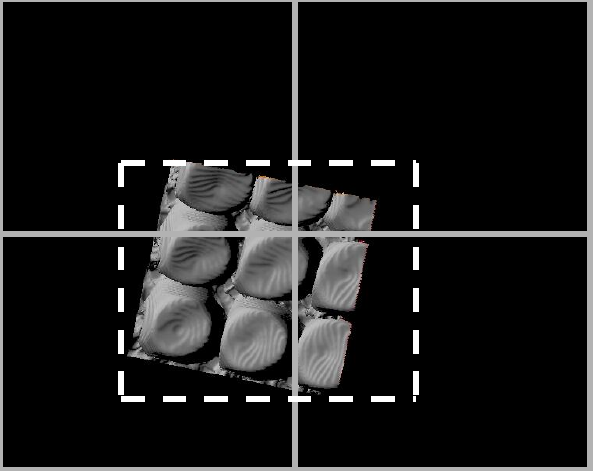
\includegraphics[width=3in]{images/FloatingViewport}
  \caption{Even though geometry may straddle tile boundaries, we may be
    able to render it all in one pass by ``floating'' the viewport.}
  \label{fig:FloatingViewport}
\end{figure}

Consider the geometry shown in Figure~\ref{fig:FloatingViewport} that
projects onto a screen space that fits within a single tile but is moved in
the horizontal and vertical directions so that it straddles four tiles.  If
the system limits itself to projecting onto physical tiles, the processor
must render and read back four images; although it could generate a single
image that contains the entire geometry with the exact same pixel spacing.
Instead of rendering four tiles, the system can \keyterm{float} the
viewport in the global display to the space straddling the tiles.  That is,
the system may project the geometry to the space shown by the dotted line
in Figure~\ref{fig:FloatingViewport} and split the resulting image back
into pieces that can be displayed directly on each tile.  Hence, the system
does not need to render any polygon more than once, and the frame buffer is
read back one time instead of four.

When a processor’s geometry fits within the floating viewport, it can cut
the rendering time dramatically.  This is most likely to happen when the
number of tiles is small compared to the number of processors and the
spatial coherency of the data is good.

The floating viewport is always enabled by default.  You can disable it by
calling \CFunc{icetDisable} with the \CEnum{ICET\_FLOATING\_VIEWPORT}
identifier.  In general, there is not much reason to turn off the floating
viewport.  The only real reason to turn off the floating viewport is to
prevent \IceT from changing the perspective matrix when in single tile
mode.  However, \IceT will change the perspective matrix anyway when
rendering with more than one tile, so any application that might render to
a tiled display should simply leave the floating viewport option on.

\index{floating~viewport|)}

\section{Active-Pixel Encoding}
\label{sec:Customizing_Compositing:Active_Pixel_Encoding}
\index{active-pixel~encoding|(}

Because each processor renders only a fraction of the total geometry, the
geometry often occupies only a fraction of the screen space in some or all
of the tiles in which it lies.  Consequently, the initial images
distributed between processors at the beginning of composition often have a
significant amount of blank space within them.  Explicitly sending this
information between processors is a waste of bandwidth.  Transferring
sparse image data rather than full image data is a well-known way to reduce
network overhead.  So far, our best method to do this has been with
active-pixel encoding.

Active-pixel encoding is a form of run-length encoding.  A traditional
run-length encoding groups pixels into contiguous groups where the color
and/or depth does not change.  However, in a practical 3D rendering, both
the color and depth change almost everywhere except in the background areas
where nothing is rendered.  To take advantage of this, images are grouped
into alternating run lengths of \keyterm{active pixels}, pixels that
contain geometry information, and \keyterm{inactive pixels}, pixels that
have no geometry drawn on them.  The active-pixel run length is followed by
pairs of color and depth values (or just one of the two if that is the only
data available)..  The inactive pixels are not accompanied by any color or
depth information.  The depth information is assumed to be of maximum
depth, and the color values are ignored since they contain no geometry
information.

There are many other ways to encode sparse images and reduce data
redundancy.  However, we are particularly enamored with our active-pixel
encoding for this application because it exhibits all of the following
properties:

\begin{description}
\item[Fast encoding]  Image encoding requires each pixel to be visited
  exactly once.  Each visit includes a single depth buffer comparison, a
  single addition, and at most one copy.
\item[Free decoding]  Processors typically perform a depth comparison as
  soon as they receive incoming data.  The depth comparison can be done
  directly against an image that is still encoded in sparse form.  In fact,
  the depth comparison can skip the comparisons for the inactive pixels.
  Thus doing depth comparisons against encoded images is often faster than
  against unencoded images.
\item[Effective compression]  During the early stages of composition when
  the largest images must be transferred, the sparse data is commonly less
  than one fifth the size of the original data.
\item[Good worst case behavior] No image with both color and depth
  information (the most common case) will ever grow by more than a few
  bytes of header information.  Images that have geometry drawn on every
  pixel will only have one run length.  Even images that alternate between
  active and inactive status for every pixel, and hence have a run length
  for every pixel, do not grow when encoded.  The number of bytes required
  to record two run lengths is equal to the number of bytes saved by not
  recording color and depth information for a single inactive pixel.  Thus,
  there is no penalty for recording run lengths of size one.  If only color
  or only depth is being recorded, it is possible to grow data in the
  pathological case where pixels alternate between active and inactive, but
  in practice background pixels are grouped and the data never really
  grows.
\end{description}

Active-pixel encoding is performed automatically during the compositing
process.  There is currently no way to turn it off.

\index{active-pixel~encoding|)}

\section{Data Replication}
\label{sec:Customizing_Compositing:Data_Replication}
\index{data~replication|(}

\sticky{\CFunc{icetDataReplicationGroup},
  \CFunc{icetDataReplicationGroupColor}}

\index{data~replication|)}

\section{Timing (and Other Metrics)}
\label{sec:Customizing_Compositing:Timing}
\index{timing|(}

Time metrics.
Message metrics.

\sticky{\CFunc{icetGet}, \CEnum{ICET\_BLEND\_TIME},
  \CEnum{ICET\_BUFFER\_READ\_TIME}, \CEnum{ICET\_BUFFER\_WRITE\_TIME},
  \CEnum{ICET\_COMPARE\_TIME}, \CEnum{ICET\_COMPOSITE\_TIME},
  \CEnum{ICET\_COMPRESS\_TIME}, \CEnum{ICET\_RENDER\_TIME},
  \CEnum{ICET\_TOTAL\_DRAW\_TIME}}

\sticky{\CEnum{ICET\_FRAME\_COUNT}, \CEnum{ICET\_BYTES\_SENT}}

\index{timing|)}
